% The Nixon Corpus -- arXiv preprint.
% Build:  make            (latexmk + pdflatex/bibtex, TeX Live on Linux)
%     or  make tectonic   (single binary, downloads packages on first run)
% Title, author and links are set in metadata.tex.
\documentclass[11pt]{article}

% =====================================================================
%  Title, author, links and draft switch. Everything below is used by
%  main.tex; nothing else needs touching to change the title, the
%  author block or the URLs.
% =====================================================================

% ---- Title ----------------------------------------------------------
\newcommand{\papertitle}{The Nixon Corpus: Speaker-Annotated Transcripts of the Nixon Tapes Using a Fine-Tuned Transformer Model}
\newcommand{\runningtitle}{The Nixon Corpus}

% ---- Author ---------------------------------------------------------
\newcommand{\authorname}{Arvin Akoopie}
\newcommand{\authororcid}{0000-0001-7833-4172}

% ---- Version line under the title ----------------------------------
\newcommand{\paperversion}{Preprint, version 1}

% ---- Links ----------------------------------------------------------
\newcommand{\repourl}{https://github.com/akoopie/nixon-corpus}
\newcommand{\releasedoi}{\textit{[Zenodo DOI to be added on deposit]}}   % replace with \url{https://doi.org/10.5281/zenodo.<record>}
\newcommand{\modelurl}{https://huggingface.co/akoopie/nixon-parakeet-tdt-0.6b-v5}

% ---- Draft switch ---------------------------------------------------
% \drafttrue shows red author notes and placeholders; \draftfalse hides
% the notes for the arXiv submission (placeholders still show).
\newif\ifdraft
\drafttrue


% ---- Page and fonts -------------------------------------------------
\usepackage[letterpaper,margin=1in]{geometry}
\usepackage[T1]{fontenc}
\usepackage[utf8]{inputenc}
\usepackage{newtxtext,newtxmath}
\usepackage{microtype}
\usepackage{setspace}
\setstretch{1.08}

% ---- Tables, figures, lists ----------------------------------------
\usepackage{graphicx}
\usepackage{booktabs}
\usepackage{tabularx}
\usepackage{multirow}
\usepackage{array}
\usepackage{siunitx}
\sisetup{group-separator={,},group-minimum-digits=4}
\usepackage{enumitem}
\setlist{itemsep=2pt,topsep=4pt}
\usepackage[font=small,labelfont=bf,skip=6pt]{caption}
\usepackage{float}
\usepackage{xcolor}
\usepackage{csquotes}

% ---- Citations and links -------------------------------------------
\usepackage[authoryear,round]{natbib}
\usepackage[hidelinks]{hyperref}
\usepackage{orcidlink}
\usepackage{xurl}
\hypersetup{pdftitle={\papertitle},pdfauthor={\authorname}}

% ---- Small helpers --------------------------------------------------
\definecolor{notecolor}{HTML}{B3261E}
% Author notes: visible in draft mode only.
\newcommand{\authornote}[1]{\ifdraft{\color{notecolor}\textsf{\footnotesize[Note: #1]}}\fi}
% Placeholders for numbers not yet filled in: always visible, so none slips through.
\newcommand{\tbd}[1]{{\color{notecolor}\textsf{[#1]}}}
\newcommand{\conv}[1]{\mbox{#1}}                 % conversation numbers, e.g. \conv{871-004}
\newcommand{\machine}[1]{\textit{``#1''}}        % quoted machine transcript
\newcommand{\pct}[1]{#1\%}
% a paragraph opening with a bold label: flush left, a small gap above (none right after a heading)
\makeatletter
\newcommand{\runin}[1]{\par\if@nobreak\else\addvspace{0.5\baselineskip}\fi\noindent\textbf{#1}}
\makeatother

\title{\papertitle}
\author{\authorname\,\orcidlink{\authororcid}}
\date{\normalsize\paperversion}

\begin{document}
\maketitle

\begin{abstract}
\noindent
Richard Nixon's secret White House taping system recorded 2,719 hours of conversation between February 16, 1971 and July 18, 1973. Hand transcription reached only the conversations needed for trials, diplomatic histories and edited selections. The Nixon Corpus transcribes all 19,426 conversations released as individual recordings: 2,206 hours, 19.0 million words, every word timed and every speech segment labeled. It rests on the first publicly documented speech recognizer fine-tuned on the tapes, a Transformer model (NVIDIA's Parakeet TDT 0.6B), and a second, independent recognizer (Whisper large-v3), reconciled by a large language model against the National Archives' subject logs, H.\,R. Haldeman's diary and the day's other conversations. Every change is a reversible edit. A voiceprint classifier names fourteen principal speakers. On 165 held-out conversations transcribed by the State Department's historians, the corpus recovers 76.1\% of words and 80.1\% of names; Whisper alone recovers 69.2\% and 60.0\%. On the 130 of them outside the classifier's training data, 92.4\% of named words carry the right speaker. Transcripts, model and code are open.
\end{abstract}

\noindent\textbf{Keywords:} Nixon White House tapes; presidential recordings; archives; speech recognition; speaker identification; large language models; Watergate

\section{Introduction}
\label{sec:intro}

On February 16, 1971, the Secret Service, at Nixon's request, began recording his conversations in the Oval Office and the Cabinet Room. Within sixteen months the system covered his office in the Executive Office Building (EOB), telephones in three rooms and Camp David. The collection ended on July 18, 1973: 2,719 hours on 4,042 reels \citep{nixonlib2019findingaid}, cataloged by the National Archives and Records Administration (NARA) as 22,723 conversations \citep{nara2024conversations} and released in stages until August 21, 2013 \citep{nixonlib2019findingaid}. It is an unusually complete record of private deliberation in a modern presidency: the opening to China, the end of the Vietnam War, the 1972 election and, conversation by conversation, Watergate.

Almost none of it had been transcribed. The Watergate Special Prosecution Force (WSPF) and the House Judiciary Committee transcribed what the prosecutions and impeachment needed \citep{wspf,hjc1974eight}; the State Department's \textit{Foreign Relations of the United States} (FRUS) printed foreign-policy conversations \citep{frus1969}; scholarly editions selected \citep{kutler1997abuse,brinkley2014nixontapes,brinkley2015nixontapes1973,prde2014nixon,dean2014defense}. Everything else had only NARA's subject logs, outlines of each conversation's topics \citep{nixonlib2010subjectlogs}. A registry of machine-readable published transcripts, compiled for this work, covered 426 conversations: 1.9\% of the catalog.

The digitized tapes have heavy amounts of static and background noise, which make transcription difficult. Microphones hidden in the Oval Office desk, beside its fireplace and in the other rooms, and taps on the telephones recorded at 15/16 inches per second, amid overlapping speakers and room noise \citep{nixonlib2019findingaid}. None of the earlier AI-assisted transcriptions \citep{fine2026easynixon,hoover2026nixon,ferguson2026unlocked} documented adapting a recognizer to the tapes. The most widely used recognizer, Whisper, conditions each word on its own previous output; it loops, skips speech and writes text over silence \citep{radford2023whisper,koenecke2024careless,baranski2025hallucination,bain2023whisperx}. Parakeet TDT, a FastConformer (a Transformer with convolution) with a transducer decoder, predicts each word chiefly from the audio \citep{xu2023tdt,nvidia2025parakeetv3}.

Here both were used. A large language model was given the two independent readings and the archive's own records and returned auditable edits; earlier systems voted between recognizers \citep{fiscus1997rover} or rewrote one recognizer's hypotheses \citep{chen2023hyporadise}. A classifier was trained to name the principal speakers instead of clustering anonymous voices \citep{bredin2023pyannote}. The contributions are the first publicly documented speech recognizer fine-tuned on the tapes, a Transformer model, a two-recognizer pipeline with archival correction, speaker labels for fourteen voices, a held-out evaluation on 165 FRUS transcripts with a corpus-wide measurement of single-model artifacts, and the open corpus, model and code.

\section{Data and methods}
\label{sec:methods}

Two recognizers transcribe each conversation: Parakeet, fine-tuned on the tapes, and Whisper, unchanged. A merge keeps Parakeet's words and attaches Whisper's reading at every disagreement. A language model corrects the merged text against the archive and returns edits. A voiceprint classifier labels the speakers (Figure~\ref{fig:pipeline}). The release keeps every layer.

\begin{figure}[t]
  \centering
  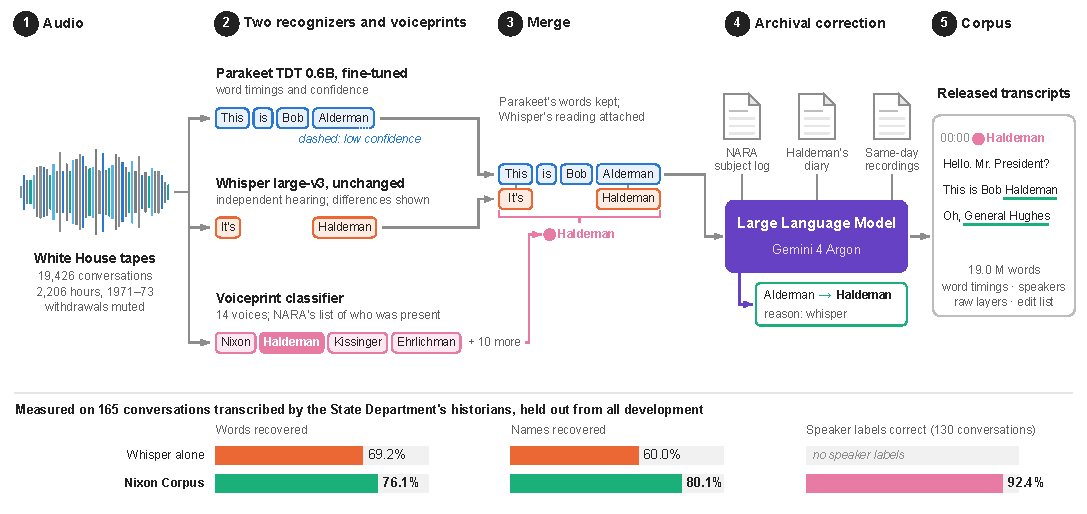
\includegraphics[width=\linewidth]{figures/fig1_pipeline.pdf}
  \caption{The pipeline, followed through one moment of the corpus: Haldeman giving his name on the telephone (\conv{018-078}, January 13, 1972). Parakeet is unsure of \machine{Alderman} (dashed); Whisper hears \machine{Haldeman}; the language model adopts Whisper's reading and cites it; the classifier names the speaker. Edits are underlined in the released transcript.}
  \label{fig:pipeline}
\end{figure}

\subsection{Sources}
\label{sec:data}

\textbf{Audio.} 19,426 conversations, February 16, 1971 to July 12, 1973, 2,206 hours, from NARA's catalog copies and the Nixon Library's older per-conversation files: 6,548 telephone conversations, 6,224 in the Oval Office, 4,435 in the EOB, 2,003 at Camp David and 216 in the Cabinet Room. That is 81.1\% of the 2,719 hours in the Nixon Library's finding aid; 44 further conversations could not be fetched, and 3,253 exist only within whole-tape files. NARA's withdrawal tones (1,242 spans in 841 conversations, 18.4 hours) were muted before transcription.

\textbf{Archive.} NARA's conversation manifest (date, time, location, participants); the subject logs, 2,383 recovered from the Library's truncated archive and matched to 94\% of conversations; and H.\,R. Haldeman's diary, 1,473 entries from January 18, 1969 to April 30, 1973 \citep{haldeman1994diaries,nixonlib2018haldemandiaries}.

\textbf{Reference transcripts}, in two strictly separated sets. \emph{Train:} everything used to build and tune the system: 60 WSPF transcripts (393,443 words) for fine-tuning, and eleven references of eight conversations (six room recordings, two telephone calls) that set the learning rate, the correction instructions and the confidence threshold. These eight were not in the fine-tuning data; five of their room recordings, the \emph{train room recordings}, are in the corpus. \emph{Test:} every FRUS document whose editors transcribed one conversation from the tape as speaker-labeled dialogue, each excerpt aligned on its own; after exclusions, 165 conversations, February 26, 1971 to June 18, 1973, 351,883 reference words (119 Oval Office, 26 telephone, 10 EOB, 5 Cabinet Room, 5 Camp David). No FRUS text reached the correction model. \emph{Registry:} NARA's WSPF and NARA transcript lists, the train references and these FRUS documents, 426 conversations. For the passages of Section~\ref{sec:cases} we also searched both Brinkley and Nichter volumes and \citet{dean2014defense}; we did not search \citet{kutler1997abuse} or the Presidential Recordings Digital Edition.

\subsection{Two recognizers}
\label{sec:asr}

\textbf{Parakeet, fine-tuned.} Parakeet TDT 0.6B v3 is a 600-million-parameter FastConformer, a Transformer with convolution, with a token-and-duration transducer decoder \citep{xu2023tdt,nvidia2025parakeetv3}; it runs at least 4.3 times faster than Whisper and does not condition on its own output. We fine-tuned it on 4,790 WSPF clips (19.9 hours, 49 conversations) force-aligned with wav2vec~2.0 \citep{baevski2020wav2vec2}, plus labels the author made by ear in twelve hours: 68 transcribed clips, 98 corrected chunks of low-confidence room audio, 38 noise clips on which the model must write nothing, and 22 stretches marked with the speaker's name, each repeated ten times. Room recall rose from 63.8\% to 68.5\% (WSPF clips), 70.0\% (plus transcribed clips), 70.7\% (plus corrected chunks) and 72.3\% for the released model, v5 (plus noise clips; learning rate $6\times10^{-5}$, AdamW, 8 epochs, NVIDIA NeMo 3.0.0, \citealp{kuchaiev2019nemo}). Decoding the corpus cost US\$8.60 of rented GPU time; 88.4\% of Parakeet's 18,274,746 words carry a confidence score.

\textbf{Whisper and the merge.} Whisper large-v3, unchanged, transcribed 19,421 conversations, a first fifth (3,891) in batches with WhisperX (settings in the repository). The merge aligns the two word by word. Agreed and Parakeet-only words stay; Whisper's reading is attached at every disagreement; Whisper fills Parakeet's silences (no Parakeet word within 0.5 seconds, mean Whisper probability at least 0.5); Parakeet words below confidence 0.01 are marked.

\subsection{Correction against the archive}
\label{sec:correct}

Recognizers turn names into ordinary words: Parakeet wrote \machine{the whole different} for Haldeman and \machine{Generally} for John Ehrlichman where Whisper heard the names. The archive often knows the name. Google's Gemini 4 Argon \citep{google2026argon} (batch interface, temperature 0.2, October 20 to 23, 2026) receives the merged transcript in 60-second blocks, with Whisper's alternatives inline and low-confidence words marked, NARA's record and subject log, and Haldeman's diary for that day and the next. Short conversations of the same day share a request, so one recording can correct another. The model keeps fillers, repetitions and grammar, never paraphrases, and marks nonsense as \texttt{[unclear]} (instructions: \texttt{src/argon.py}). It returns edits: block, words replaced, replacement, confidence and the main evidence (\texttt{whisper}, \texttt{nara}, \texttt{diary}, \texttt{day}, \texttt{context}, \texttt{knowledge} or \texttt{sound}). 98.5\% of edits are located and applied by exact match; every edit is marked and reversible. All conversations with words were corrected except six. Cost: 57.3 million input and 19.4 million output tokens, US\$154.13 at the batch price (US\$0.07 per audio hour), or US\$308.26 at the standard price at which Google billed the batches completed by October 21.

\subsection{Speakers}
\label{sec:speakers}

A logistic-regression classifier on frozen WeSpeaker ResNet-34 embeddings \citep{wang2023wespeaker}, normalized by room type, names fourteen voices (Nixon, Kissinger, Haldeman, Ehrlichman, Colson, Dean, Ziegler, Mitchell, Rogers, Shultz, Haig, Woods, Connally, Butterfield) or \enquote{other}. Training: 24,656 clips from 902 conversations, from WSPF speaker turns, from two-person recordings on which Nixon was confidently ruled out (bringing in Kissinger, Haig, Rogers and others), and from the author's 22 marks. Each Whisper segment of at least 1.5 seconds is scored among the people NARA lists as present and named at probability 0.7 or more.

\subsection{Evaluation}
\label{sec:eval}

Hypotheses and references are normalized with Whisper's English normalizer \citep{radford2023whisper}, cut to their shared stretch and aligned word by word. Measures: word recall, $1-(S+D)/N$; word error rate, $(S+D+I)/N$; name recall and name precision over the reference's names (words capitalized mid-sentence at least twice and in at least 80\% of their uses; a wrong name absent from the reference is not counted); recall on Nixon's turns and on replies of four words or fewer. Test intervals: 95\% bootstrap over conversations, paired between layers. The test set informed no decision and shares no conversation with the train set. Of 231 FRUS conversations we excluded 44 not in the corpus (43 released only within whole-tape files, one released after our list was built), 9 the author had heard, labeled or corrected, 7 parallel recordings of excluded conversations and 6 whose audio holds a different conversation. FRUS text can be in the correction model's pretraining data, so the merged layer, untouched by any language model, is reported beside the corrected layer.

\section{Results}
\label{sec:results}

\subsection{Accuracy}
\label{sec:res-acc}

\runin{Fine-tuning worked.} On the six train room recordings, none of which were in the fine-tuning data, fine-tuning raised Parakeet's word recall from 63.8\% to 72.3\%, a paired gain of 8.5 points (95\% interval 5.0 to 10.8; Figure~\ref{fig:accuracy}c). Recall on Nixon's own words rose from 49.3\% to 64.9\% and on short replies from 32.2\% to 46.7\%, while WER fell from 39.0\% to 31.3\%.

\runin{The corpus beat Whisper on held-out data.} On the 165 FRUS conversations, the corrected layer recovered 76.1\% of reference words, against 69.2\% for Whisper alone (Table~\ref{tab:main}, Figure~\ref{fig:accuracy}). Of the 6.9-point gain (interval 6.3 to 7.7), 4.5 points came from fine-tuned Parakeet and 2.4 from correction. The corpus was more accurate than Whisper on 160 of the 165 conversations. The gap between the two recognizers was largest on Nixon's own words, which Parakeet v5 recovered at 71.6\% and Whisper at 63.6\%, and on short replies, at 50.8\% and 36.0\%. By location, the corrected layer recovered 85.6\% of words at Camp David, 83.7\% on the telephone, 76.6\% in the Oval Office, 76.5\% in the Cabinet Room and 49.3\% in the EOB (Figure~\ref{fig:accuracy}d).

\runin{Correction supplied the names.} Parakeet v5 recovered 60.2\% of names and Whisper 60.0\%. Correction raised name recall by 19.8 points, to 80.1\%, with no loss of precision: of the reference names the corrected layer displayed, 90.3\% were right, against 89.0\% for Whisper alone.

\begin{table}[t]
\centering
\caption{Accuracy of each corpus layer (\%). Train: the five train room recordings in the corpus (48,189 reference words). Test: 165 held-out FRUS conversations (351,883 reference words), with 95\% bootstrap intervals over conversations in brackets.}
\label{tab:main}
\small
\setlength{\tabcolsep}{4pt}
\begin{tabular}{@{}l ccc ccc@{}}
\toprule
 & \multicolumn{3}{c}{Train (five room recordings)} & \multicolumn{3}{c}{Test (165 FRUS conversations)} \\
\cmidrule(lr){2-4}\cmidrule(lr){5-7}
Layer & Word recall & WER & Names & Word recall & WER & Names \\
\midrule
Whisper large-v3 alone & 57.2 & 45.8 & 48.8 & 69.2 {\footnotesize[67.4, 70.7]} & 42.0 & 60.0 {\footnotesize[57.0, 62.8]} \\
Parakeet v5 alone & 72.4 & 31.3 & 73.0 & 73.7 {\footnotesize[72.0, 75.1]} & 38.1 & 60.2 {\footnotesize[57.2, 63.2]} \\
Merged (no language model) & 72.5 & 31.1 & 73.1 & 73.7 {\footnotesize[72.1, 75.2]} & 37.9 & 60.3 {\footnotesize[57.2, 63.2]} \\
Corrected & \textbf{73.9} & \textbf{29.6} & \textbf{81.2} & \textbf{76.1} {\footnotesize[74.5, 77.6]} & \textbf{35.1} & \textbf{80.1} {\footnotesize[77.3, 82.5]} \\
\bottomrule
\end{tabular}
\end{table}

\begin{figure}[t]
  \centering
  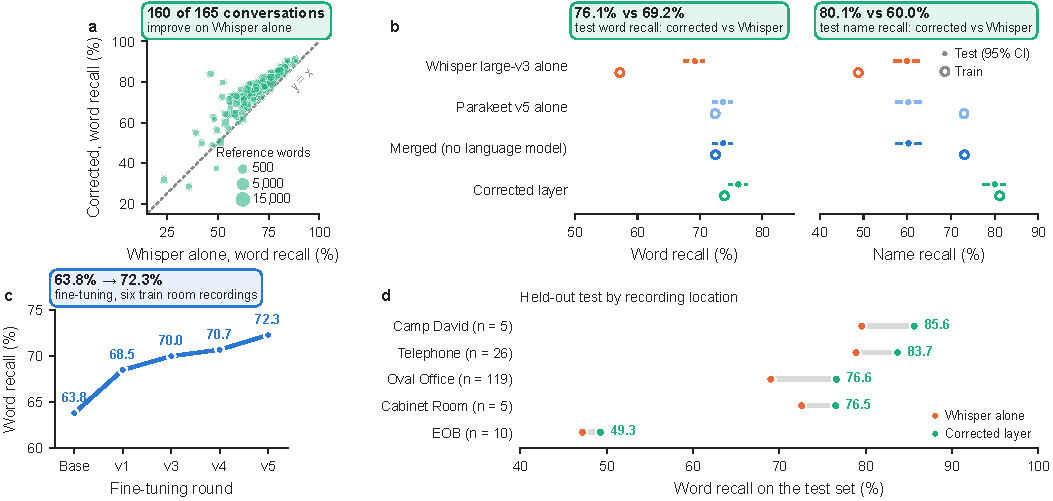
\includegraphics[width=\linewidth]{figures/fig2_accuracy.pdf}
  \caption{Accuracy. \textbf{a},~Word recall of each of the 165 held-out FRUS conversations, Whisper alone against the corrected layer (marker size: reference words). \textbf{b},~Word and name recall of each layer on the test set (filled, 95\% intervals) and the five train room recordings in the corpus (open). \textbf{c},~Fine-tuning: pooled word recall on the six train room recordings, by round. \textbf{d},~Test word recall by recording location, Whisper alone and corrected.}
  \label{fig:accuracy}
\end{figure}

\subsection{Artifacts of single-model transcription}
\label{sec:res-artifacts}

\runin{Whisper alone looped, dropped speech and wrote over silence} (Figure~\ref{fig:artifacts}). Its output contained 2,613 repetition loops, the same words written over and over, in 1,463 conversations (55,140 words); Parakeet v5 produced 105 loops and the released corrected layer 265. When run in batches with WhisperX \citep{bain2023whisperx}, the configuration of earlier machine transcriptions of the tapes \citep{fine2026easynixon}, Whisper also discarded speech: wherever WhisperX wrote nothing for 20 seconds or more, Parakeet still transcribed speech. These 3,973 stretches held 5.2\% of Parakeet's words in those conversations, and in 2,869 of them Parakeet wrote at least 60 words a minute, a rate that only real speech produces. Over NARA's muted withdrawals, Whisper wrote 1,882 words in 422 conversations, typically \enquote{you} every 30 seconds, while Parakeet wrote 131 words over the same silence. Across the corpus, Whisper also wrote 987 stock phrases such as \enquote{thank you for watching}. No word inside a muted passage was kept in the release. Each recognizer also heard words that the other missed, and both were therefore kept in the corpus.

\begin{figure}[t]
  \centering
  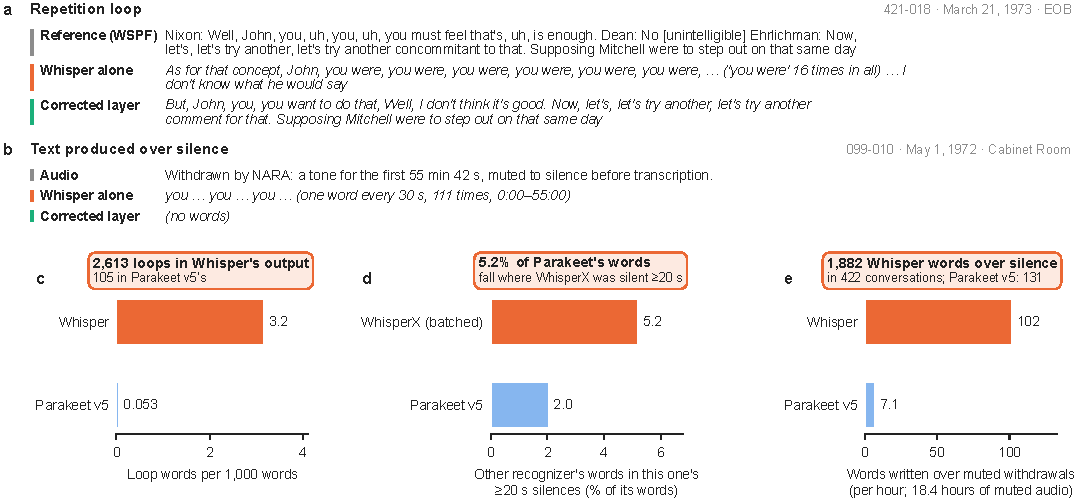
\includegraphics[width=\linewidth]{figures/fig3_artifacts.pdf}
  \caption{Artifacts of Whisper-only transcription, from the corpus's own Whisper layer. \textbf{a},~A repetition loop (\conv{421-018}): Whisper repeated \enquote{you were} sixteen times and lost Ehrlichman's turn; the corrected layer recovered it. \textbf{b},~Text over silence (\conv{099-010}): across a 55-minute withdrawal, muted before transcription, Whisper wrote \enquote{you} every 30 seconds; the corrected layer held no words. \textbf{c},~Loop words per 1,000 words, whole corpus. \textbf{d},~Dropped speech: the other recognizer's words that fell in this one's silences of 20 seconds or more (WhisperX: the batched fifth). \textbf{e},~Words written over muted withdrawals per hour of muted audio.}
  \label{fig:artifacts}
\end{figure}

\subsection{What the second reading and the correction added}
\label{sec:res-correct}

On the Test set, at least one recognizer was right on 79.5\% of reference words, 6.0 points more than Parakeet alone on the same words, and correction recovered 2.4 of those points. \textbf{The second reading drove the gain.} On the five train room recordings in the corpus, correction gained 405 reference words when given Parakeet's text alone, 564 when Whisper's readings were added and 712 when low-confidence words were also marked; before the corpus run, 340 edits helped and 20 hurt. \textbf{Same-day context corrected across recordings.} On April 9, 1971, Parakeet's \machine{want Dr. Burns, uh, Marjorie Burns? I'm pleased to call} (\conv{476-021}) was corrected to \machine{Find Dr. Burns, Arthur Burns, I placed a call}, the words of the telephone recording of the same moment (\conv{001-061}); the author confirmed both by ear. \textbf{Edits cited their evidence.} Of the corrected names in the Test set, 42.8\% cited Whisper's reading and 34.8\% the subject log; only 4.6\% cited the model's own knowledge.

\subsection{Speakers}
\label{sec:res-speakers}

On the 130 Test conversations outside the classifier's training data (220,664 aligned words), the classifier named the speaker of 68.4\% of words, and \textbf{92.4\% of named words carried the speaker named in the FRUS transcript}. For the fourteen voices it was trained on, the figure was 95.9\%: 94.9\% for Nixon over 78,305 named words and 97.5\% for Kissinger over 50,743 (Figure~\ref{fig:corpus}c). Its cross-validated balanced accuracy, the average of its accuracy on each voice, was 87.2\%.

\section{The corpus}
\label{sec:corpus}

Release 1.1 (Table~\ref{tab:corpus}, Figure~\ref{fig:corpus}) is one JSON record per conversation: NARA's metadata and subject log, audio sources, withdrawn spans, speaker segments, and every word with its timing, speaker, confidence and source (Parakeet, both recognizers, a Whisper fill, a model edit or a correction by ear). Each edit keeps what it replaced and why. Plain-text transcripts and the raw recognizer outputs ship with it. A browsing application in the repository presents the corpus by day, conversation and person and plays each transcript in sync with the audio; no language model writes its text.

\begin{table}[t]
\centering
\caption{The Nixon Corpus, release 1.1.}
\label{tab:corpus}
\small
\begin{tabularx}{\linewidth}{@{}l X@{}}
\toprule
Conversations & 19,426 (February 16, 1971 -- July 12, 1973), 17,343 with words \\
Audio & 2,206 hours: 6,548 telephone, 6,224 Oval Office, 4,435 EOB, 2,003 Camp David, 216 Cabinet Room \\
Words & 18,994,348, each with start and end time, source and confidence; every model edit marked and reversible \\
Speakers & 63\% of words named; of 1,461 hours of scored speech, 1,023 named (Nixon 637, Haldeman 99, Kissinger 79) \\
Context & NARA date and location for every conversation, participants for all but 35, subject log for 94\% \\
Format & JSON (gzip), plain text, metadata table, raw layers, checksums; 776\,MB \\
\bottomrule
\end{tabularx}
\end{table}

\begin{figure}[t]
  \centering
  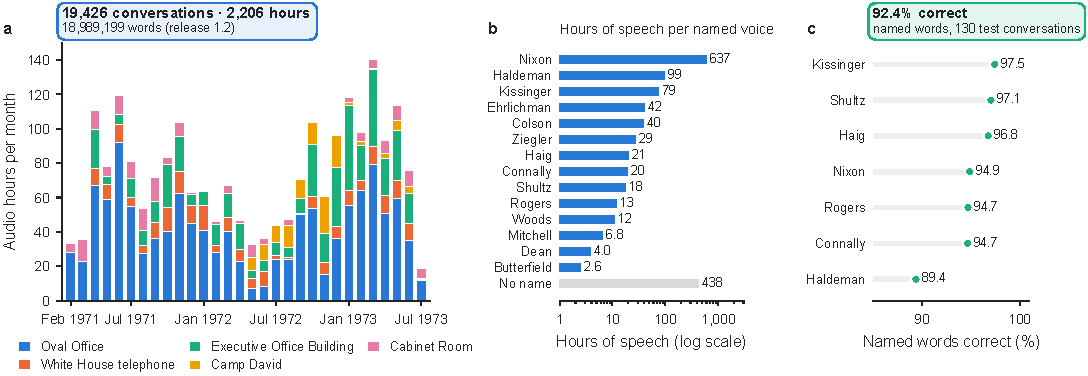
\includegraphics[width=\linewidth]{figures/fig4_corpus.pdf}
  \caption{The corpus. \textbf{a},~Audio hours per month by recording location, February 1971 to July 1973. \textbf{b},~Hours of speech per named voice (segments named at probability 0.7 or more; log scale) and the 438 scored hours without a name. \textbf{c},~Named words correct on the 130 held-out test conversations outside the classifier's training data, for voices with at least 200 named words.}
  \label{fig:corpus}
\end{figure}

\section{Three passages}
\label{sec:cases}

Every quotation below is word for word from the released corrected transcript, with its punctuation and standard capitalization, and was checked by the author against the audio.

\subsection{The corpus matched a participant's transcript: \conv{871-004}, March 7, 1973}
\label{sec:case-dean}

With L. Patrick Gray's confirmation as FBI director going badly \citep{crs2018fbi}, Nixon told John Dean he wanted friendly senators to question Gray under oath about what J. Edgar Hoover had told him. Dean printed the passage from his own transcription \citep[Conversation No.~871-4]{dean2014defense}:

\begin{quote}\small
\textbf{Dean (2014):} \enquote{I'm going to make him lie, because I think Gray's not handling himself well. What he said yesterday with regard to the fact that this `jolly well' bullshit \ldots\ that it was highly improper for you to be present \ldots}

\textbf{This corpus (5:26--5:48):} \machine{I told him that Hoover had told me, and I'm going to make him lie because I think Gray's not handling himself well. What he said yesterday with regard to the fact that, it was, that, you know, this jolly well bullshit and all that sort of thing that you were, that it was highly improper for you to be present.}
\end{quote}

These are the recognizers' own words: the correction step made no edit here. Over the surrounding minutes the merged layer shared 95 of its 1,288 five-word sequences with Dean's text, against 10 to 20 for unrelated stretches. Dean printed what he selected; the corpus holds the whole conversation, including Nixon's question at 4:55 about the FBI's 1968 \machine{electronic surveillance of Vice President Agnew is phone when he was in Phoenix}. The documented check concerned calls from Albuquerque \citep{johnson1968deloach,hughes2014chasing}: the recognizer heard Nixon correctly, and the slip was his.

\subsection{The cover story in Nixon's words: \conv{916-019}, May 11, 1973}
\label{sec:case-916}

Eleven days after Haldeman and John Ehrlichman resigned, and days after Vernon Walters testified that they had sought the CIA's help in stopping an FBI investigation \citep{brinkley2015nixontapes1973}, Nixon met Haldeman and Alexander Haig in the Oval Office. At 10:20 Nixon (confirmed by the author's listening) told Haldeman how Ehrlichman's account of the June 23, 1972 meeting with the CIA's leaders should go:

\begin{quote}\small
\machine{Now, my point is, John's story should be perfect, should be, and I hope you talked to John. John's story is perfect. John should say his only concern was the whole CIA involvement and so forth and wanted to be sure that the, this investigation of Watergate didn't get out, as he put it, didn't get out of hand. [\ldots] Getting out of hand had to do with exactly what's now happening. Yeah. Which is unloading all this Pentagon papers. Investigation type stuff, the leak, the plumbers operation type stuff, the, Exactly. Wiretapping of the reporters and, and staff members type stuff.}
\end{quote}

\enquote{John} is Ehrlichman: the conversation placed \machine{Ehrlichman and me} at the meeting and said \machine{Dean was not there} and that \machine{Ehrlichman did do all the talking}. Parakeet transcribed these words where Whisper wrote nothing; the correction step did not touch them. At 13:00 Nixon named his concern and Haldeman answered (\machine{paint a} is the author's correction by ear of \machine{faint}):

\begin{quote}\small
\textbf{Nixon:} \machine{I, I don't need to paint a picture. I just want to be sure that John doesn't indicate that the President directed him to get Walters to get Gray to turn this off and set up a phony story}\\[2pt]
\textbf{Haldeman:} \machine{John would never indicate that. [\ldots] What the President tells us to do is not, not public, public consumption.}
\end{quote}

It was Nixon who, on June 23, 1972, told Haldeman that the CIA's leaders \enquote{should call the FBI in and say that we wish for the country, don't go any further into this case, period!} \citep{wspf1974exhibit1}. No published transcript of this exchange\footnote{Easy Nixon's unreviewed machine transcript of \conv{916-019} \citep{fine2026easynixon} does not contain it.} was found in the registry, in either Brinkley and Nichter volume, in \citet{dean2014defense} or on the Nixon Library's and Miller Center's pages for the conversation; \citet{kutler1997abuse} and the Presidential Recordings Digital Edition were not checked.

\subsection{The ordinary record, and further leads}
\label{sec:case-ordinary}

Most of the tapes are routine, and the corpus captures that too. On March 14, 1972, after John Mitchell's ITT testimony, Nixon telephoned Charles Colson and tried out a line, \machine{this is a smear a day Congress rather than a law day of Congress}; Colson laughed, and they agreed to use it (\conv{021-068}). No subject log records such exchanges. Further leads were surfaced by ranking corpus windows outside the registry for politically charged terms; each was heard and confirmed by the author (Table~\ref{tab:leads}).

\begin{table}[t]
\centering
\caption{Further leads, with prior-publication checks. Three other candidates were already in print \citep{dean2001rehnquist,dean2014defense}.}
\label{tab:leads}
\small
\begin{tabularx}{\linewidth}{@{}l l X X@{}}
\toprule
Conversation & Date, place & Passage & Prior publication \\
\midrule
\conv{789-006} & Sept.~30, 1972, Oval Office & \machine{super apathy among the blacks}, called \machine{just exactly where you want it} before the election & Not in the registry or \citet{brinkley2014nixontapes} \\
\conv{233-010} & Dec.~6, 1972, Camp David & \machine{make Sweden the black post. I want a black for Sweden} & Not in \citet{brinkley2014nixontapes}; in earlier machine transcripts \citep{fine2026easynixon} \\
\conv{690-011} & Mar.~21, 1972, Oval Office & An ambassadorship and a request to \machine{get at least 150 out of it} & Not in \citet{brinkley2014nixontapes}; in earlier machine transcripts \citep{fine2026easynixon} \\
\bottomrule
\end{tabularx}
\end{table}

\section{Limitations and conclusion}
\label{sec:conclusion}

\runin{Limitations.} The corpus is a machine transcript and a finding aid. It recovered 76.1\% of test reference words, and 49.3\% in the EOB, so every quotation should be checked against the audio, to which every word is linked. FRUS editors chose the test excerpts; a test set drawn at random from the corpus would measure the whole record. Correction depends on a proprietary model, but its edits are marked and reversible. Voices without a class of their own were sometimes given a trained speaker's name (16.9\% of their test words). Withdrawn passages stay muted, and passages about private persons call for care in republication.

\runin{Conclusion.} Two recognizers that err differently, reconciled against the archive's own records, turn the released Nixon tapes into a searchable, speaker-labeled text of 19.0 million words. On held-out conversations this text recovered 76.1\% of words and 80.1\% of names, against 69.2\% and 60.0\% for Whisper alone. It tells a historian where to listen, with measured accuracy, word timings and speaker labels that neither the subject logs nor earlier machine transcripts provide.

\section*{Declarations}
\addcontentsline{toc}{section}{Declarations}

\paragraph{Data, code and model availability.} The corpus (release 1.1) is archived at \releasedoi, with a data card that documents its format, coverage and limitations. The code for the pipeline, the evaluation and the browsing tool, the scripts that rebuild the public-domain reference transcripts, and the correction instructions (\texttt{src/argon.py}) are at \url{\repourl}. The fine-tuned recognizer is at \url{\modelurl}. The corpus viewer is available at \url{\siteurl}, where the transcripts can be read and searched with the audio playing alongside.

\paragraph{License and citation.} The transcripts, annotations and model weights are released under CC BY 4.0; attribution should take the form of a citation of this paper and of the release. The model derives from NVIDIA's Parakeet-TDT-0.6B-v3 (CC BY 4.0; \citealp{nvidia2025parakeetv3}). The code is MIT-licensed. The recordings, NARA's metadata and the government transcripts are public domain; please credit NARA and the Richard Nixon Presidential Library and Museum as their source.

\paragraph{Use of AI tools.} AI systems were used as components of the pipeline (the speech recognizers, the speaker-embedding network and the correction model, Gemini 4 Argon, as reported above) and as assistants: the software was written, the analyses were run and the manuscript was drafted with the help of an AI coding assistant (Claude, Anthropic). The author designed the study, directed all analyses, made the research decisions, performed all annotation and listening, and takes full responsibility for the content of this paper.

\paragraph{Acknowledgments.} The author thanks the National Archives and Records Administration and the Richard Nixon Presidential Library and Museum, whose archivists preserved, reviewed, described and released the recordings, and whose subject logs and conversation manifest made this work possible.

\paragraph{Competing interests and funding.} The author declares no competing interests. The work received no external funding; computing costs were paid by the author.


\bibliographystyle{plainnat}
\bibliography{references}

\end{document}
